\newpage
\section{Timer}

\begin{figure}[h!]
	\centering
	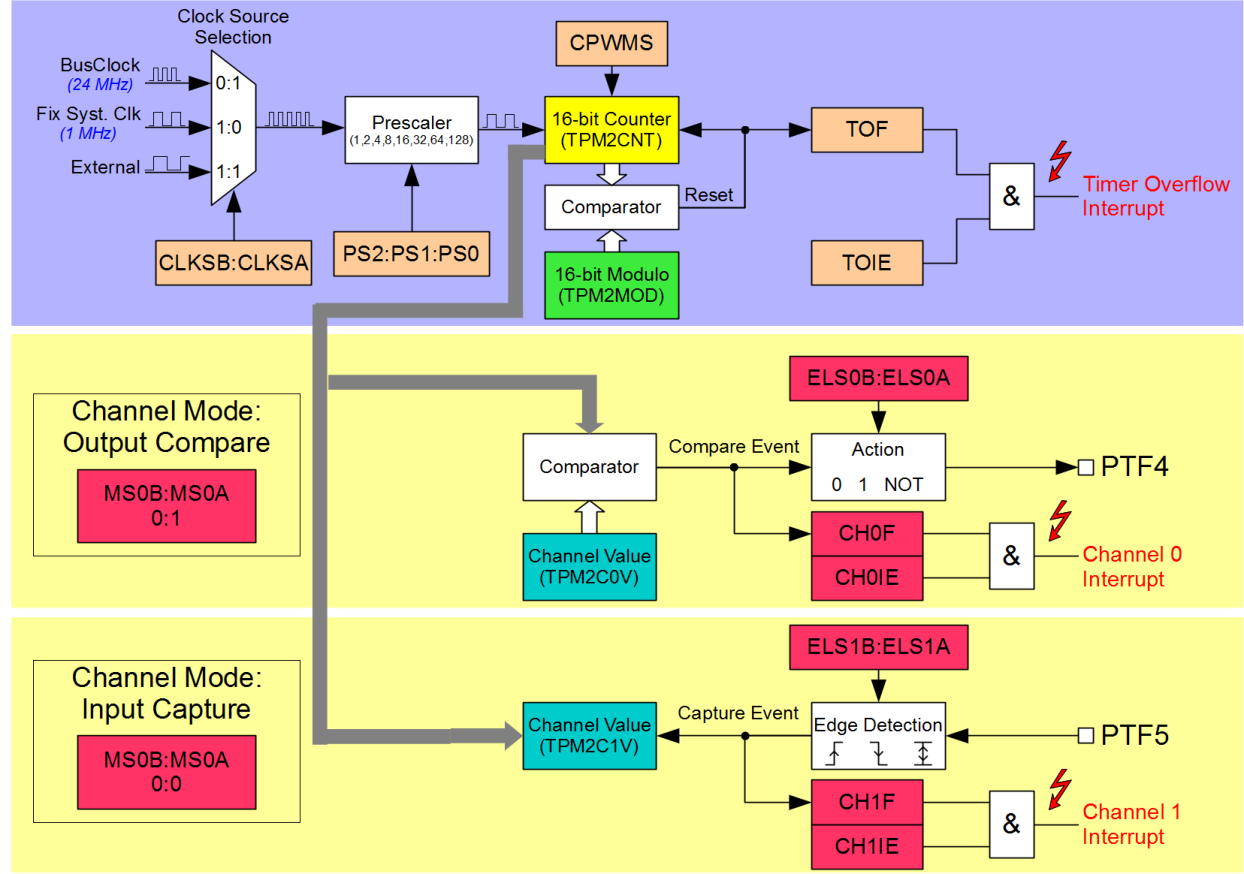
\includegraphics[width=1\textwidth]{../fig/timer.pdf}

	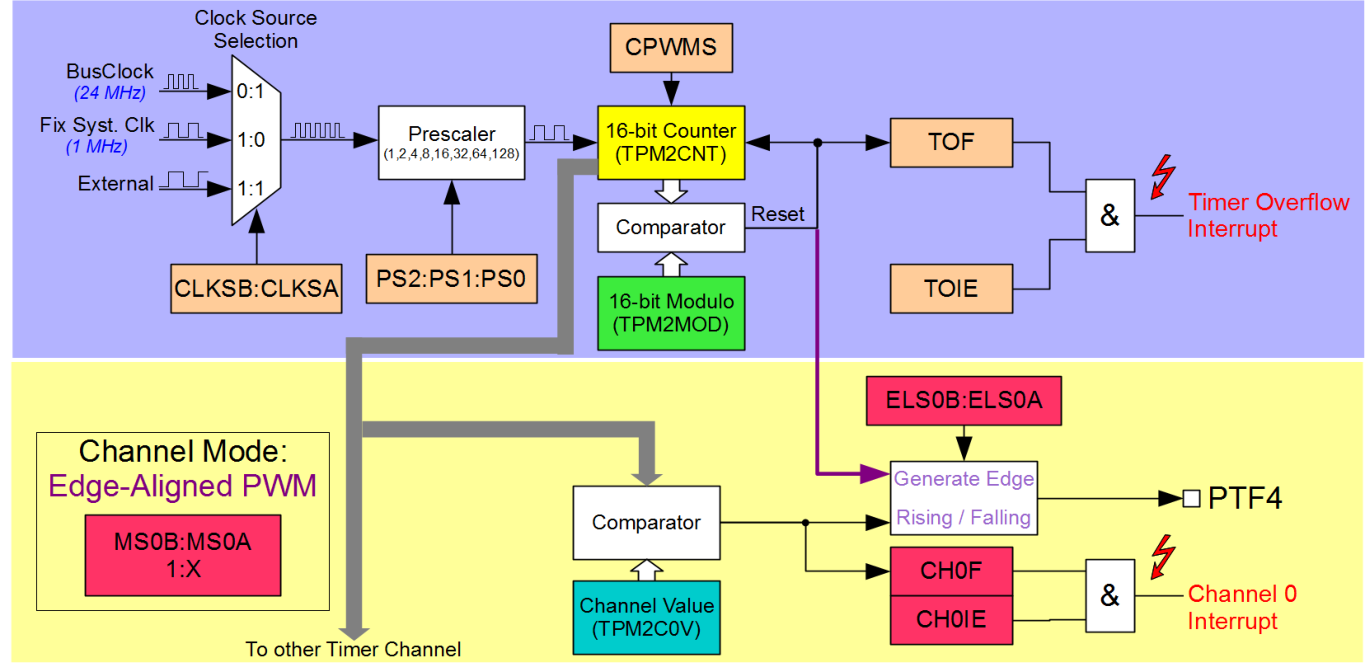
\includegraphics[width=1\textwidth]{../fig/pwm.pdf}
	\caption{Übersicht der Timer-Register}
\end{figure}

\subsection{PWM}
Ein PWM-Signal kann auf drei verschiedene Arten implmentiert werden
\begin{enumerate}
	\item Timer aufsetzen mit MODULO = Periodendauer, 
		ChannelValue = Implsdauer, Modul-Pin setzen/rücksetzen mit
		CompareEvent Einstellung (ohne ISR)
	\item Timer aufsetzen mit MODULO = Periodendauer,
		ChannelValue = Impulsdauer, beliebigen Pin setzen/rücksetzen
		mit ISR
	\item Timer aufsetzen mit MODULO = DEFAULT, ChannelValue ist
		abwechselnd TimerCounter+Impulszeit und
		TimerCounter+(Periodendauer-Inpulszeit)
\end{enumerate}

\begin{figure}[h!]
	\centering
	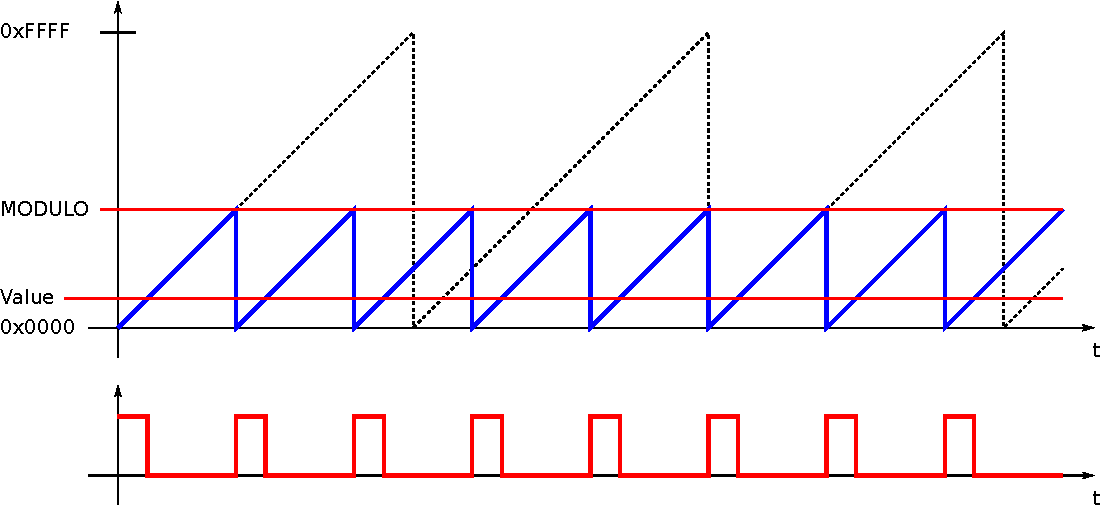
\includegraphics[width=1\textwidth]{../fig/pwm_01.pdf}
	\caption{PWM mit MODULO und ChannelValue}
\end{figure}

\begin{figure}[h!]
	\centering
	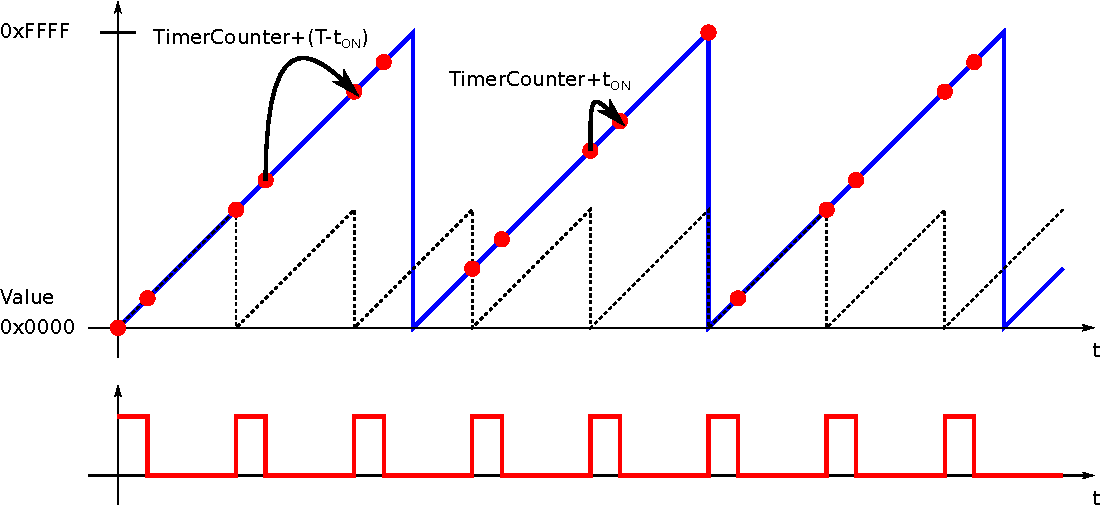
\includegraphics[width=1\textwidth]{../fig/pwm_02.pdf}
	\caption{PWM ohne MODULO}
\end{figure}

\newpage
\subsection{Beispiele}

\subsubsection{Output Compare}
\lstinputlisting[firstline=19, lastline=95, title=main.c]{../src/timer_oc/Sources/main.c}
\lstinputlisting[firstline=60, lastline=60, title=Project.prm]{../src/timer_oc/Project_Settings/Linker_Files/Project.prm}

\begin{comment}
\newpage
\subsubsection{PWM}
\lstinputlisting[firstline=19, lastline=70, title=main.c]{../src/timer_pwm_led/Sources/main.c}
\lstinputlisting[firstline=59, lastline=59, title=Project.prm]{../src/timer_pwm_led/Project_Settings/Linker_Files/Project.prm}
\end{comment}

\newpage
\subsubsection{PWM mit MODULO, VALUE, ohne ISR}
\lstinputlisting[firstline=19, title=PWM - Variante 1]{../src/timer_pwm_var1/Sources/main.c}

\newpage
\subsubsection{PWM mit MODULO, VALUE und ISR}
\lstinputlisting[firstline=19, title=PWM - Variante 2]{../src/mep_timer_pwm_var2/Sources/main.c}

\newpage
\subsubsection{PWM ohne MODULO}
\lstinputlisting[firstline=19, title=PWM - Variante 3]{../src/timer_pwm_var3/Sources/main.c}
